\documentclass[tikz, border={5pt, 15pt}]{standalone}

\usetikzlibrary{shapes}

\begin{document}

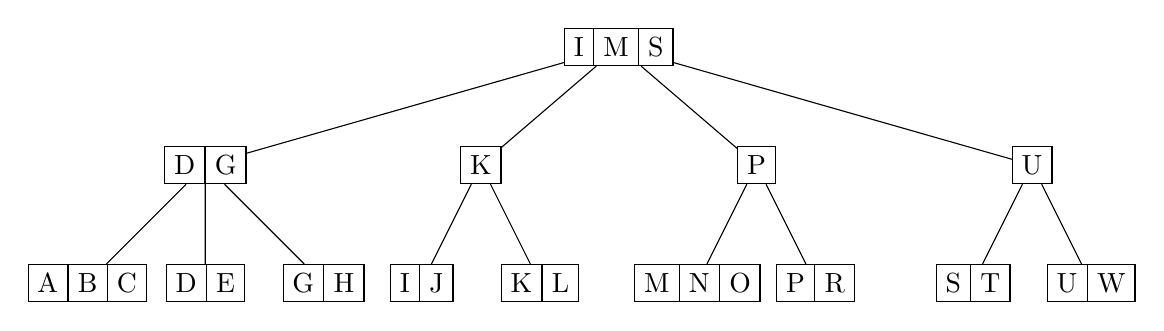
\begin{tikzpicture}
\tikzstyle{bplus-node}=
[
	draw, rectangle split,
	rectangle split horizontal,
	rectangle split ignore empty parts
]
\tikzstyle{every node}=[bplus-node]

\tikzstyle{level 1}=[sibling distance=35mm]
\tikzstyle{level 2}=[sibling distance=15mm]

\node {I \nodepart{two} M \nodepart{three} S} [-]
	child {node {D \nodepart{two} G}
		child {node {A \nodepart{two} B \nodepart{three} C}}
		child {node {D \nodepart{two} E}}
		child {node {G \nodepart{two} H}}
	}
	child {node {K}
		child {node {I \nodepart{two} J}}
		child {node {K \nodepart{two} L}}
	}
	child {node {P}
		child {node {M \nodepart{two} N \nodepart{three} O}}
		child {node {P \nodepart{two} R}}
	}
	child {node {U}
		child {node {S \nodepart{two} T}}
		child {node {U \nodepart{two} W}}
	}
;
\end{tikzpicture}

\end{document}
